\chapter{仿冒应用检测框架\mytool}
\label{chp:framework_prototype}

前两章分别从仿冒应用基本特征与仿冒应用开发者的行为特征入手,对仿冒应用开展实证研究,获取了仿冒应用命名、大小、投放偏好等特性,也说明了当下的应用市场并未对仿冒应用进行有效拦截。
基于实证研究的发现,作者设计了仿冒应用检测框架\mytool 。
通过使用\mytool ,应用市场方可在大规模应用中实现对已知正版应用及其对应仿冒样本的快速鉴别,有效检查出开发者上传的仿冒或正版应用,提高应用市场方的审核速度。
本章将先阐述\mytool 的设计与实现,再进行系统实验并解析实验结果。

\section{框架设计与实现}

\subsection{整体设计}
\mytool 是一个轻量的仿冒应用检测框架,基于已知的正版特征对输入的应用集进行自定义筛选。
应用市场方可将其用于大规模的Android应用检测,自动筛选出其中的正版应用与潜在仿冒应用,再结合人工审查,完成对仿冒应用的验证、归类和对可疑行为的提取,感知潜在的威胁。

\begin{figure}[htbp]
    \centering
    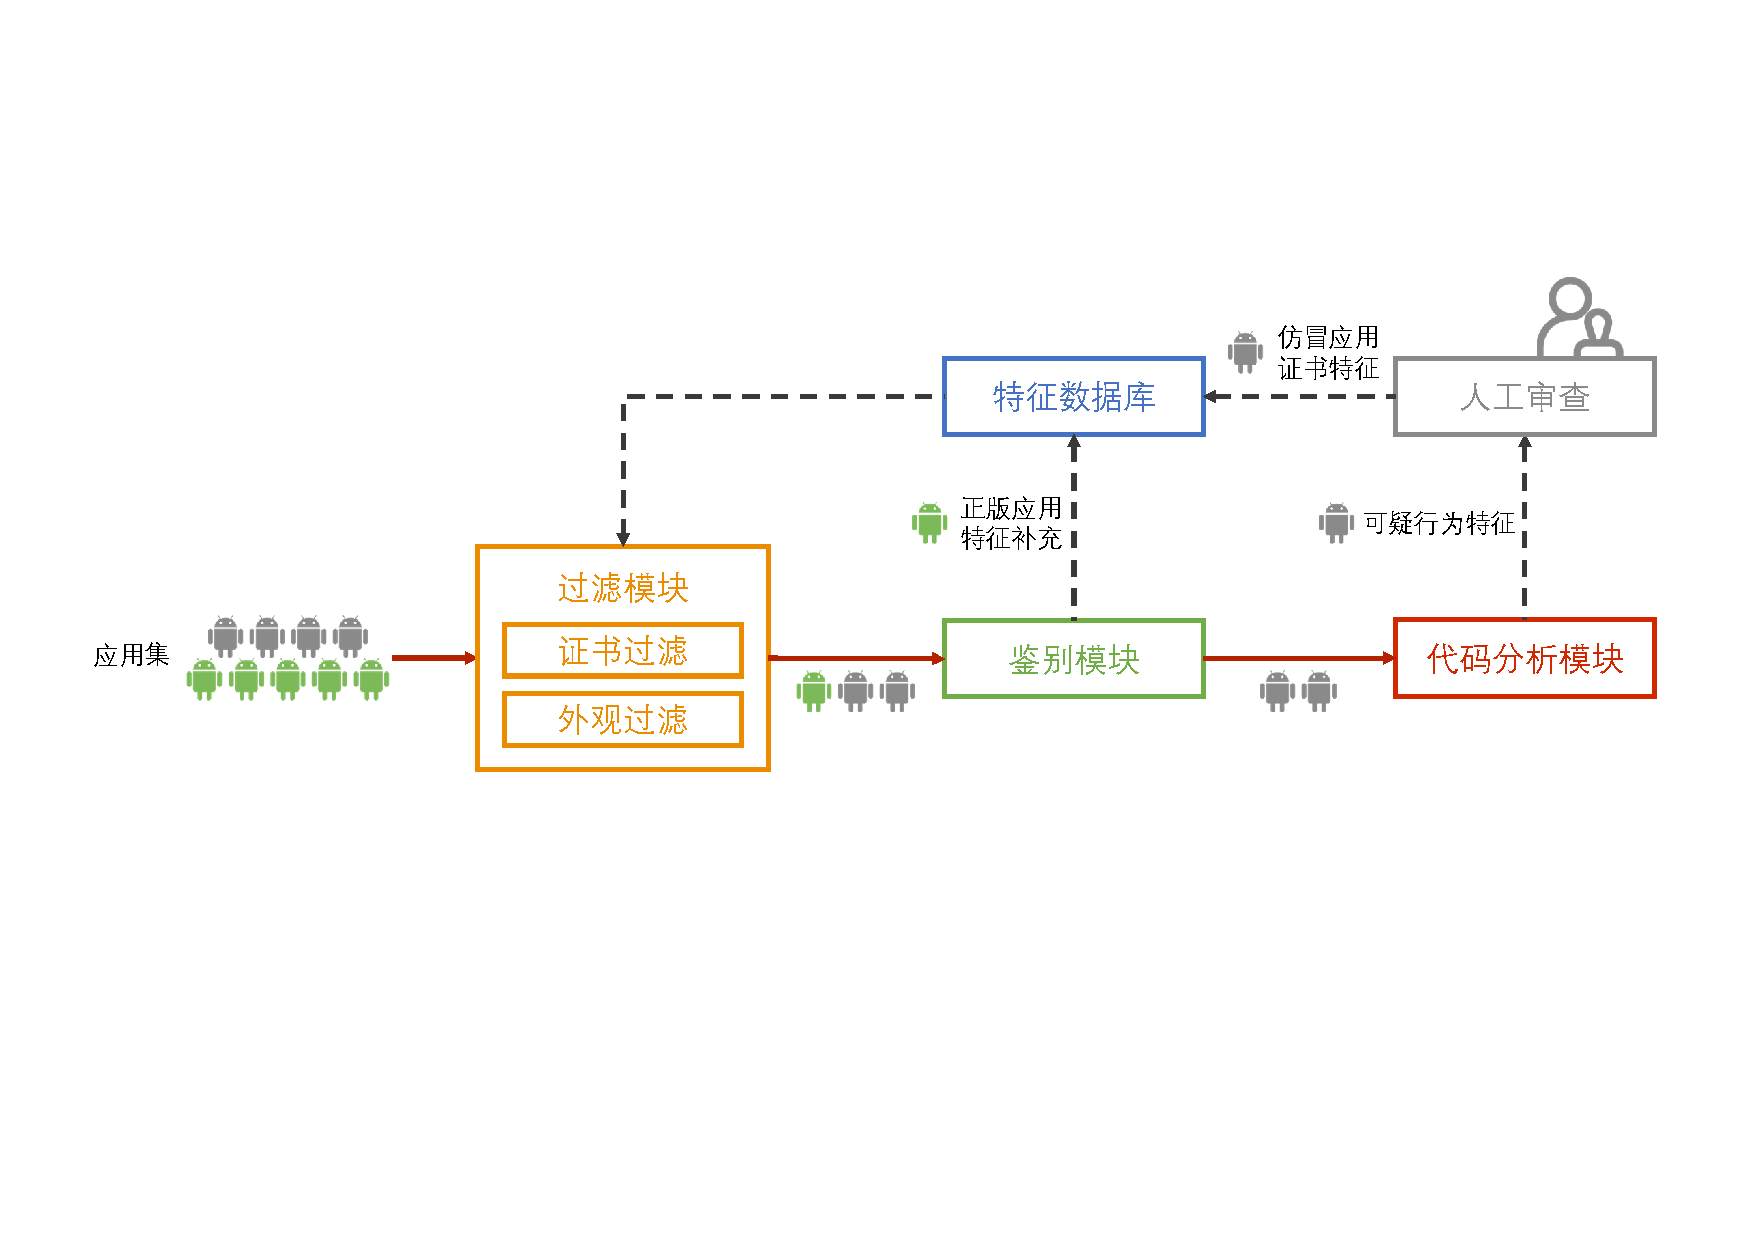
\includegraphics[width=\textwidth]{./Figures/edwin-fakerevealer-detector}
    \caption{\mytool 整体流程}
    \label{fig:Workflow_detector}
    \vspace{-3mm}
\end{figure}

\autoref{fig:Workflow_detector}展示了\mytool 的整体工作流程,框架主要分为\textbf{\componentA} 、\textbf{\componentB} 、\textbf{\componentC}、\textbf{\componentD} 和\textbf{\componentE} 五个部分。
\componentE 为存储应用特征的数据库,用户在使用前,需要先在\componentE 中输入部分正版应用特征信息和其他相关信息(如开发者黑名单)作为先验知识。
\mytool 以Android应用集为输入,先利用\componentA 对应用集进行初筛,过滤与正版应用不相关或相似度低的应用,降低后续检测与人工审核的压力。
之后,\componentB 提取应用样本的证书信息进行仿冒鉴别。
被判别为正版的应用样本的外观特征将被提取进\componentE 中以加强后续检测;被判别为仿冒的应用样本则会进入\componentC 被提取行为信息。
\componentC 提取应用中的静态分析数据(如应用代码中的方法信息、类信息等),构造方法调用图,分析应用的行为信息;此外,应用样本的基本信息也会被提取,方便后续展示。
之后,\componentC 分析涉及敏感API调用(如打电话、收发短信等)的应用行为,其中的可疑行为会被记录,汇总后分发到\componentD 环节复核。
Android应用面对的业务场景是十分复杂的,类似的方法调用行为在不同业务场景下会有截然不同的含义,因此现阶段仍需\componentD 确认应用的API调用是否可疑或具有恶意。
结合框架给出的应用信息和方法调用关系,应用市场审核人员可对仿冒应用进行快速判别,提高审核效率。
最后,在\componentD 环节确认为仿冒应用或恶意应用的样本的证书特征将被加入\componentE ,由同一开发者证书签署的其他应用在未来的检测中会在\componentA 阶段被直接拦截。

框架基于Python 3编写。

\subsection{\componentA }
\componentA 分为两部分,分别为\textbf{证书过滤}和\textbf{外观过滤}。
在面向规模较大的应用集输入时,\componentA 有三个主要功能:
其一为通过应用证书信息比对,筛出黑名单开发者的应用,拒绝将其上架;
其二为通过将输入的应用与已知正版应用匹配,将与已知正版应用无关的输入过滤,减少后续检测压力;
其三为对输入的应用分类,以便在\componentB 中根据分类进行对应的正版检测。

证书过滤指应用进入框架后,将先被提取证书信息,与\componentE 中已有的开发者黑名单比对。
若应用证书于黑名单内,该应用将被直接拒绝上架,流程结束。
证书信息比对部分的开发者黑名单由应用市场方自行维护,其中应包括已知仿冒开发者的证书信息与用于在Android Studio等开发环境调试的debug证书信息。
应用市场也应定期与其他各应用市场共享黑名单信息,防止\fullref{chp:discoveries_basic}中发现的仿冒应用开发者在多个市场中上传应用、利用debug证书上传应用等风险再次产生。

外观过滤则再分为应用名匹配与应用图标匹配两部分。
在应用名匹配部分,判断输入应用是否与某一已知正版应用匹配的依据源于\componentD 中的正版应用命名模式。
一个正版应用的命名模式由若干个特征点通过逻辑运算(与、或运算)连接而成,每个特征点为该正版应用的命名特征。
一个特征点可由正则表达式表示,也可以是应用名长度范围。
由\fullref{chp:discoveries_basic}总结可得,仿冒应用的命名与对应的正版应用十分接近,因此应用市场方也可给出某正版应用名与相似度阈值作为特征点,加入该正版应用的命名模式。
比如,由观察可得\textit{爱奇艺}的应用名常有更改,但总会以``爱奇艺''起始,可用\textit{app\_name(``爱奇艺\*'')}表示该类特征;
而\textit{similarity(``开心消消乐'', 0.6)}则会将与``开心消消乐''相似度大于等于0.6的应用名纳入匹配范围。

应用图标匹配部分,应用市场方需要先为已知正版应用配置一个图标和相似度阈值作为比较标准,\componentA 获取输入应用图标后,对两者进行相似度计算,若相似度大于等于阈值,则认为两者相似。
现有的主流图像相似度算法可分为四类,分别为严格判别算法、直方图比较、哈希算法和特征匹配法。
严格判别算法即对两图片的像素点作严格一一比对的算法,速度较快,但敏感度太高,鲁棒性并不好,只适用于严格判定图像全等的领域;
直方图比较则将两张图片的直方图数据归一化后进行相似度比较;
哈希算法会先为每张图片生成一个哈希串,再通过哈希串之间对比实现图像相似度对比,可理解为将图像相似度转化为字符串相似度计算的算法;
特征匹配法则通过提取图像中的特征点,计算特征点的特征向量后,比对不同图像的特征向量进行相似度比对。
在对比了哈希算法与特征匹配法的性能后,本框架采用了特征匹配算法计算图像相似度。

具体实现方面,证书信息在利用apktool对应用拆包后,使用JDK的keytool工具提取,APK中的图标文件具有固定路径,其提取也在apktool拆包后进行;
应用名提取由Android SDK中的aapt命令行工具对APK文件进行解析后,从解析结果中截取获得;
字符串匹配的相似度由两者之间的编辑距离与给出应用名的长度之比计算,特征匹配算法使用了图像的GIST(Generalized Search Tree)特征~\cite{torralba2003context}。

匹配之后,应用名和应用图标均被判定为与已知正版应用相似的样本会被打上对应标签(标记样本与哪个已知应用类似),进行后续的仿冒鉴别。
不被\componentA 判定为与已知正版应用相关、且应用证书不在开发者黑名单中的应用样本将进入应用市场方原有审核流程,而非由本框架判定是否仿冒应用或可否上架。

\subsection{\componentB }
\componentB 根据\componentA 的标签对应用进行进行仿冒判别,判别依据为样本内的证书指纹信息。
由\secref{sec:signature}可知,Android应用的签名信息可在大部分场景下指向应用的最后修改者,但恶意开发者仍可利用在2017年被揭露的Janus漏洞,对使用V1机制签名的APK进行篡改。

\begin{figure}[htbp]
    \centering
    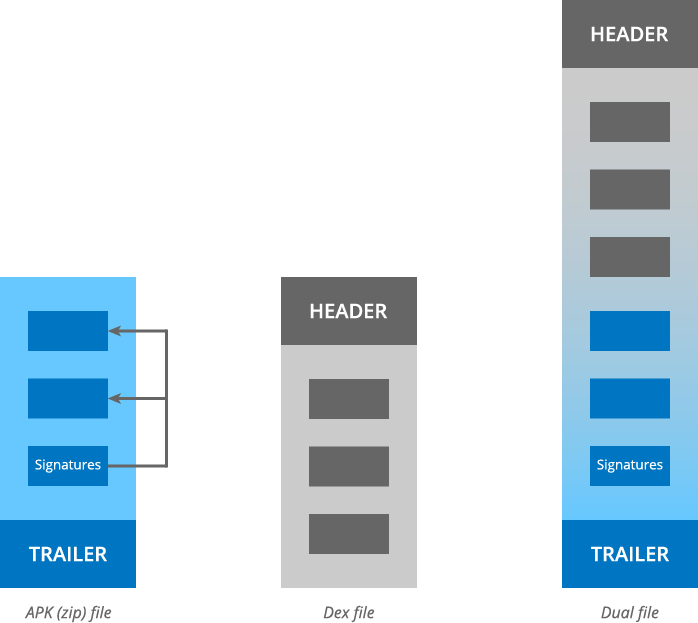
\includegraphics[width=0.7\textwidth]{./Figures/edwin-janus}
    \caption{Janus漏洞原理}
    \label{fig:how_janus_works}
    \vspace{-3mm}
\end{figure}

\autoref{fig:how_janus_works}\footnote{本图源于网络资料~\cite{CVE_2017_13156}}展示了Janus漏洞的工作原理。
在安装APK文件时,虚拟机先从APK的尾部(Trailer一端)读取校验签名信息(图中的Signature部分),校验成功后再从文件头部对APK文件进行解析和安装。
然而,Android系统的dex虚拟机同时支持对dex文件和apk文件的读取和执行。
若在APK文件头部拼接一个dex文件,虚拟机在完成新文件的尾部校验之后、跳转到文件头部对新文件进行解析安装时,将直接执行拼接于头部的dex文件,导致系统被攻击。

因此,对于使用V2、V3机制签名的应用,本框架直接利用应用的证书信息判别其是否仿冒应用;对于使用V1机制签名的应用,框架除验证证书信息外,还使用另一种手段确保应用未被攻击。
根据dex文件格式,每个dex文件的前8个字节为Magic number字段,内容为固定值``dex$\backslash$n035$\backslash$0'';而APK文件本质上为ZIP格式的压缩文件,也具有固定格式,文件头部的前4个字节内容为16进制的``504b0304''。
基于上述格式对文件头部前4个字节的内容读取判断,可鉴别应用是否损坏或被使用Janus漏洞攻击。

在本模块中被鉴别为正版应用的样本,其图标特征将被提取进\componentE 中以加强后续检测;若应用样本被认定为仿冒应用,则会进入\componentC 被提取代码信息。
利用Janus漏洞篡改应用的开发者将被直接加入\componentE 的开发者黑名单中。

\subsection{\componentC }

经过\componentA 和\componentB 对应用筛选鉴别后,\componentC 对应用进一步提取信息。
本模块提取的数据有两类,一类为应用的基本数据,另一类为应用的代码数据。
基本数据指应用的包名、构建应用使用的Android API版本、应用版本名称、应用版本号、应用大小、应用中声明使用的权限和证书指纹信息,以上信息可通过现有工具直接读取APK文件获取。
代码数据则指利用代码分析技术获取的数据。借助静态分析技术,\componentC 可从代码获取应用中的模块结构信息,包括应用中的类信息、各类中包含的方法信息、调用关系和应用写在\textit{AndroidManifest.xml}文件中的配置。
本模块在提取数据后,进一步分析调用关系,获取声明但未被使用过的敏感权限、敏感API调用链等信息,作为审核依据流转至\componentD 。

具体来说,\componentC 借助Androguard~\cite{Androguard},对应用中的dex文件进行反编译,获取反编译后的代码信息。
对dex文件反编译得到的Java代码中,按类的定义者区分,可将应用代码中包含的类分为三种类型,分别为系统类,用户自定义类和第三方类。
系统类指Android官方提供的开发框架中的类,如Android四大组件之一Activity的基类\textit{android.app.Activity};
第三方类指并非由Java语言本身提供、也并非开发者在项目中编写的类,通常包含于开发者引入的第三方库代码中,如游戏类应用常用Unity提供的第三方库作为游戏引擎;
用户自定义类指应用开发者在开发该应用时,于项目中自行编写定义的类(包括继承系统类的自定义类)。
Android Studio对应用项目进行编译打包时,会将部分系统类、项目中的所有第三方类和所有用户自定义类都编译进dex中。
对dex文件反编译出的所有代码进行解析会产生一定性能影响,也不利于应用间区分。
因此,\componentC 在处理时先使用Libradar~\cite{ma2016libradar}将系统类剔除和识别第三方类,一则减少后续分析的数据量,二则避免第三方类中的敏感API调用对后续分析产生影响。

\begin{algorithm}[!ht]
    \tablewuhao
    \caption{敏感API调用关系排查算法}
    \label{alg:dfs}
    \KwIn{ $permissions\_API$,列表,Android权限与API映射关系}
    \KwIn{ $decleared\_permissions$,列表,包含正版应用及其信息键值对}
    \KwOut{ $redundant\_permission$,集合,应用声明的冗余权限}
    \KwOut{ $calling\_sequence$,集合,分析后的敏感API的调用序列}
    \SetKwProg{Fn}{Function}{:}{}

    \Fn {iterSearcher($permissions\_API, decleared\_permissions$)} {

        $redundant\_permission \gets \emptyset$;

        \For {$permission \in decleared\_permissions$} {

            $flag \gets$ 0;

            \For {$API \in permissions\_API[permission]$} {

                $callers \gets $getCallers($API$);

                \If {not $caller$.is\_empty} {

                    $flag \gets$ 1;

                }

                \For {$caller \in callers$} {

                    $cache$ = PermissionCallAnalysis($caller$, $\emptyset$);

                    $calling\_sequence$.update($cache$);

                }
            }

            \If {$flag$ = 0}{

                $redundant\_permission$.add($permission$);
            }

        }
        \KwRet{$redundant\_permission$, $calling\_sequence$};

    }
\end{algorithm}

除了类信息,\componentC 还提取应用中的方法信息协助之后的人工审核。
提取的方法信息包括用户自定义的所有方法以及Android框架中较为敏感的方法调用信息。
用户自定义方法通过对Androguard中获得的用户自定义类进行方法分析获取:\componentC 遍历所有自定义类,获取其定义的每个方法,再将类名与方法名组合为二元组\textit{<class\_name, method\_name>},作为该方法在应用中的唯一标识保存;
敏感方法调用信息则以自底向上的方法进行排查。

在基本数据获取阶段,\componentC 通过aapt获得了构建应用的Android API版本和应用中声明使用的权限,而Androguard附带了各Android API版本中API与权限的映射关系。
结合以上信息可获取在某应用中可能会被调用到的敏感API,详情可见\autoref{alg:dfs}。
对于应用声明的每个权限,先通过映射关系查出其对应的敏感API列表;
对于每个敏感API,算法遍历应用中的各个用户自定义类和第三方类,排查应用中是否有对该敏感API的调用(第6行)。
如果有,则对调用该API的方法层层回溯,分析出敏感API的调用序列(第11行),具体流程见后文。
对于某个已声明的权限,如果其对应的全部敏感API均没有调用记录,则可对应两种情况:
一,该权限为由开发者声明的冗余权限,可能会被恶意应用利用,造成额外风险;
二,开发者通过Java反射机制调用了与权限对应的敏感API,导致该调用无法被静态分析扫描到。
无论是哪种情况,都可能对用户安全产生隐患,也可被视作风险点,因此\componentC 会记录该权限为冗余权限(第13行)。

\begin{algorithm}[!ht]
    \tablewuhao
    \caption{调用链回溯算法}
    \label{alg:trackback}
    \KwIn{ $cur\_method$,当前遍历的方法}
    \KwIn{ $itered\_methods$,集合,已遍历的方法}
    \KwOut{ $calling\_sequence$,集合,分析后的敏感API的调用序列}
    \SetKwProg{Fn}{Function}{:}{}

    \Fn {PermissionCallAnalysis($cur\_method, itered\_methods$)} {

    $calling\_sequence \gets \emptyset$;

    $callees \gets$ getCallees($cur\_method$);

    $callers \gets$ getCallers($cur\_method$);

    $cur\_seq \gets  []$;

    \For {$callee \in callees$} {
        \If{$callee$.is\_permission\_related\_API}{
            permission = $callee$.get\_related\_permission();

            $cur\_seq$.add($<callee, permission>$);
        }
    }

    \For {$caller \in callers$} {
        \If{$caller$.is\_self\_defined $\&\& caller \notin itered\_methods$} {
            $itered\_methods$.add($caller$);

            $res \gets$ PermissionCallAnalysis($caller, itered\_methods$);

            \For {$sequence \in res$} {

                $calling\_sequence$.add($sequence$ + $cur\_seq$);

            }
        }
    }
    \If {$calling\_sequence$.is\_empty $\&\&$ not $cur\_seq$ != []}{

    $calling\_sequence$.add($cur\_seq$);

    }

    \KwRet{$calling\_sequence$};

    }

\end{algorithm}

在实现对敏感API调用链的回溯分析时,有两点挑战如下:
第一点是方法调用路径中可能会出现调用环;第二点是敏感API及其前序方法可能存在多个调用者。
前者指同一个方法多次出现在调用链中(如某方法多次递归调用自身后再调用敏感API),容易导致工具在进行调用链回溯时出现死循环;
后者让调用链成为了一棵以敏感API为根节点的调用树,树上的每个节点为一个方法,节点之间的有向边表示方法之间的调用关系。
方法调用并不是一个线性过程,各方法之间灵活的相互调用导致了以上两点挑战。

为应对以上两点挑战,\componentC 采用DFS算法和集合进行调用链回溯处理,具体可见\autoref{alg:trackback}。

对个某个方法,\componentC 先借助Androguard获取其所有被调用者(第3行)和调用者(第4行)。
如果被调用者中包含与权限相关的API,则将$<API, permission>$(即该API和其对应的权限)加入现有调用序列中(第6到9行)。
之后,对每个调用者,若其之前未被分析过,且其为用户自定义方法,则递归调用方法$PermissionCallAnalysis$回溯以该方法为起始点的权限相关API调用序列(第10至15行)。
对于方法是否被调用过的判断可以保证之前分析过的方法不再被重复分析,避免死循环的产生;
遍历调用者和递归调用$PermissionCallAnalysis$保证了所有调用者均可被回溯,若某方法没有被其他自定义方法调用、或是其调用者已经全被被分析过,则该方法为回溯终点。

分析结束后,\componentC 将应用信息汇总,流转至\componentD 。

\subsection{\componentD }

应用市场的审核人员在本模块对仿冒应用进行风险评估和确定。
尽管本框架的前三个模块自动化地进行了仿冒应用的判别和应用行为信息的获取,但应用的业务场景十分复杂,相同的API调用链在不同业务场景下可以有截然不同的含义(如``获取设备位置信息并上传至服务器''在导航软件中是必要的,而其他应用的相同行为可能会侵犯用户隐私),因此人工审查仍然不可避免。
此处的人工审查有两个作用,其一是对被鉴定为仿冒的应用进行确认,排除误报信息,并根据误报情况修正\componentA 中不同部分的匹配阈值;其二是对仿冒应用的行为进行风险评估,根据应用行为的风险大小决定对应用和对应开发者的处理。
如果一个样本仅在外观上模仿正版应用,但应用行为没有可疑之处,应用市场可驳回该次上架请求,要求开发者修正应用名与图标后重新申请上架;
然而,若样本的确包含高风险行为甚至包含恶意代码,应用市场除了拒绝上架该应用,还可以对应用开发者作封禁处理,将应用中的证书指纹信息加入\componentE 的黑名单中,在未来的检测中直接拦截相同证书签署的应用。

% 最后,\componentC 汇总各样本文件的检测结果并输出。
% 虽然框架在应用筛选、数据提取和规则判定上都实现了自动化,免去了审核方安装、运行应用或手动反编译APK等人工成本,但在应用量较大时,误判风险是无法避免的,需要由人工对结果进行复核确认。
% 每项规则都通过的样本被判别为正版应用,在经过人工确认后,其在\componentB 中被抽取的数据将会作为特征被存入\componentD 中。

% 同样需要人工的还有规则梳理部分。
% \secref{sec:func_and_behavior}显示,仿冒应用开发者在对不同类型的应用进行仿冒时,会有不同的行为特征,如\texttt{开心消消乐}的仿冒版本实际运行状况与正版相似,\texttt{王者荣耀}的仿冒则多为简单的拼图、壁纸等应用。
% 因此,人工审查的另一个作用在于观察被判定为仿冒应用的样本,为正版应用制订个性化规则,提高检测的准确率。

\section{系统实验}

上节介绍了框架的设计与实现,本节将介绍针对框架的实验设计和结果分析。

\subsection{数据收集}

为检验\mytool 的有效性,作者重新从Janus平台上收集了286个应用样本对\mytool 进行测试。
286个应用样本包含了采集自5个热门应用的255个样本和随机采集的31个噪声样本,详细分布可见~\autoref{table:exp_data_count}。

\begin{table}[htbp]
    \renewcommand{\arraystretch}{1}
    \footnotesize
    \centering
    \caption{\mytool 实验样本来源}
    \vspace{1mm}
    \begin{tabular}{l ccc}
        \toprule
        {\bf 来源应用} & {\bf 正版数量} & {\bf 仿冒数量} & {\bf 总计} \\
        \midrule
        抖音           & 32             & 18             & 50         \\
        开心消消乐     & 51             & 27             & 78         \\
        保卫萝卜       & 21             & 15             & 36         \\
        贪吃蛇大作战   & 14             & 29             & 43         \\
        WiFi万能钥匙   & 2              & 46             & 48         \\
        噪声应用       & N/A            & N/A            & 31         \\
        \bottomrule
    \end{tabular}
    \label{table:exp_data_count}
\end{table}

噪声样本用于检验\mytool 是否准确地在不产生应用误报(将无关应用识别为与已知应用相关的应用)的前提下,找到与已知应用有关的Android应用。
在\componentA 的图标匹配部分,算法效果可能受已知样本数影响。
框架为了消除该影响,实验在不同类别的应用中采用了不同的正版/仿冒数量比例作对比。

\subsection{实验与结果}

进行本组实验的设备搭载了Intel i5-8250 CPU与24GB内存。
由于已知研究中,与仿冒应用直接相关的资料较贫乏,对比实验以近似研究提出的工具(\secref{sec:study_repackaging}中的CodeMatch~\cite{CodeMatch})作为比较对象。
CodeMatch是利用第三方库信息检测重打包应用的工具,用户在使用前需先将已知第三方库信息加入数据库中。
工具先扫描APK文件获取代码,然后排除其中的已知第三方库,通过计算、比对剩余代码的哈希值进行重打包判断。
根据本文定义,重打包应用也属于一种仿冒应用,因而可采用CodeMatch进行对比实验。

\noindent{\bf 实验1:工具有效性验证}

本实验以上节的286个应用样本组成测试集。
\mytool 在使用前需先配置正版应用相关信息,作者从测试集的5种正版应用中各取2个正版样本,提取其应用图标中的特征作为先验知识存入数据库中,图标匹配的相似度阈值均设置为0.8,余下276个样本输入\mytool 进行测试。

\begin{table}[htbp]
    \renewcommand{\arraystretch}{1}
    \footnotesize
    \centering
    \caption{有效性实验结果}
    \vspace{1mm}
    \begin{tabular}{l ccccccc}
        \toprule
        \bf{来源应用}                  & \makecell[c]{\bf 正版样本识别数                                                     \\ \bf (TN)} & \makecell[c]{\bf 仿冒样本识别数 \\ \bf (TP/rbg} & \makecell[c]{\bf 仿冒样本识别数 \\ \bf (TP/gray)} & {\bf FN} & \makecell[c]{\bf FP \\ \bf (rbg)} & \makecell[c]{\bf FP \\ \bf (gray)} \\
        \midrule
        抖音                           & 30                              & 15        & 17       & 0      & 3       & 1       \\
        \rowcolor{gray!15}开心消消乐   & 49                              & 24        & 24       & 0      & 3       & 3       \\
        保卫萝卜                       & 19                              & 10        & 11       & 0      & 5       & 4       \\
        \rowcolor{gray!15}贪吃蛇大作战 & 12                              & 29        & 29       & 0      & 0       & 0       \\
        WiFi万能钥匙                   & 0                               & 32        & 30       & 0      & 14      & 16      \\
        \rowcolor{gray!15}噪声应用     & 0                               & 0         & 0        & 0      & 0       & 0       \\
        {\bf 总计}                     & {\bf 110}                       & {\bf 110} & {\bf111} & {\bf0} & {\bf25} & {\bf24} \\
        \bottomrule
    \end{tabular}
    \label{table:exp_1_effectiveness}
\end{table}

\autoref{table:exp_1_effectiveness}展示了\mytool 对6种应用的辨识结果。
表中的``rgb''和``gray''分别对应图标匹配时采用的不同模式;``TP'',``TN'',``FP'',``FN''分别对应\textit{True Positive},\textit{True Negative},\textit{False Positive}和\textit{False Negative},用于描述实验结果。
因\mytool 用于鉴别仿冒应用,实验的``Positive''被设置成鉴别为仿冒的样本数目,``Negative''为鉴别为正版的样本数目(即``非仿冒样本''的数目)。

``rgb''模式表示采用包含rgb信息的原图像进行特征采集,``gray''模式表示在采集特征前先对图标进行灰度化处理。
在rgb模式下,每个像素点的色彩由``r'',``g'',``b''三个值表示,每个值的值域为$[0, 255]$,而在gray模式下,一个像素点的色彩只需用一个值域同为$[0, 255]$的值表示其灰度,因此在gray模式下进行的特征运算和比较速度更快。
结果表明,两种模式下的检测效果相当,gray模式甚至略优于rgb模式。
综合效果与运算速度,gray模式更适合本框架使用。
另外,\mytool 在两种模式下均能正确辨认所有正版样本,因此\autoref{table:exp_1_effectiveness}中的TN与FN不再分模式列出数据。

从实验数据看,\mytool 的平均准确率($Precision = \frac{TP}{TP+FP}$)分别为81.48\%(rgb模式)和82.22\%(gray模式),召回率($Recall = \frac{TP}{TP+FN}$)均为100\%,F1值($2\times \frac{Precision \times Recall}{Precision + Recall}$)则分别为89.80\%(rgb模式)和90.24\%(gray模式),无正版应用错判记录,整体可用性较好,在个别应用(\textit{贪吃蛇大作战})下甚至可以识别出所有仿冒样本。
\mytool 不对正版错判的原因有两个,一个是于\secref{sec:signature}中介绍的Android签名机制,另一个是\componentB 将正版图标特征反馈回特征数据库的机制。
前者保证持有正版开发者证书的应用不会被误判为仿冒应用,后者保证\mytool 对新图标有一定容错性。

\begin{figure}[htbp]
    \centering
    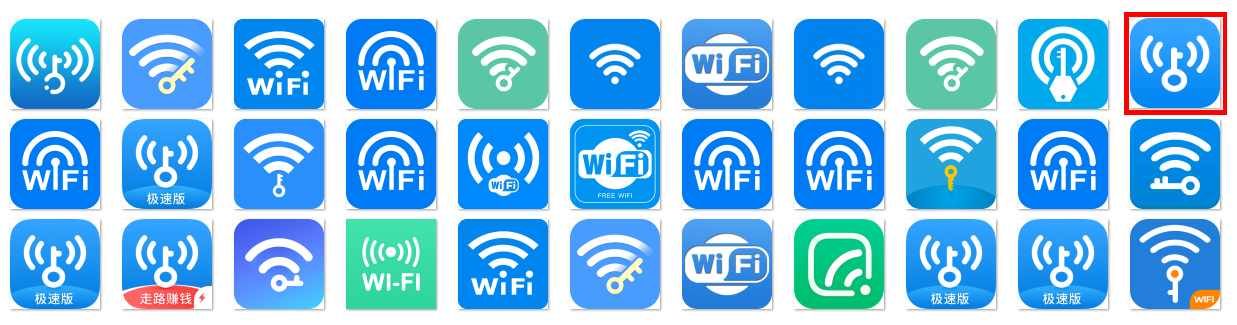
\includegraphics[width=\textwidth]{./Figures/edwin-exp-comparison}
    \caption{正版与仿冒版\textit{WiFi万能钥匙}图标}
    \label{fig:exp_comparison_icon}
    \vspace{-3mm}
\end{figure}

然而,在\textit{WiFi万能钥匙}应用下,\mytool 的鉴别能力较差,46个仿冒样本中有16个样本未被拦截。
人工确认结果显示,该部分样本均因为图标匹配未达阈值而被误判。
\autoref{fig:exp_comparison_icon}展示了\textit{WiFi万能钥匙}对应的部分仿冒应用图标,正版图标于右上角由红色边框标出。
该结果表明图标匹配算法仍有改进空间。

为确保\mytool 仅对已知应用样本生效,测试集还包含了31个随机搜集的应用样本(噪声应用),该组样本的图标和应用名均与已知的5种应用不类似,用于测试\mytool 是否会对未收录的应用类别产生误报。
数据显示,31个噪声应用均未被判定为正版或仿冒,\mytool 具有一定抗干扰能力。

\noindent{\bf 实验2:对比实验}

本组实验用于比较CodeMatch与\mytool 在分析应用时的有效性,分为时效性对比与准确性对比。
实验采用\textit{WiFi万能钥匙}一组的样本作为实验对象。
由于CodeMatch并不能直接判断应用是否为仿冒应用,因此作者直接以2个正版样本与46个仿冒样本组成的92个应用对作为CodeMatch的输入,检查46个仿冒应用中是否存在正版应用的重打包样本。
\mytool 组以实验1中的gray模式实验数据作为结果与CodeMatch对比。

\begin{table}[htbp]
    \renewcommand{\arraystretch}{1}
    \footnotesize
    \centering
    \caption{对比实验结果}
    \vspace{1mm}
    \begin{tabular}{l ccc}
        \toprule
        {\bf 工具名}    & 平均用时  & 判断出的仿冒应用(或重打包应用)数 \\
        \midrule
        {\bf CodeMatch} & 51.86分钟 & 0                                  \\
        {\bf \mytool }  & 1.13分钟  & 30                                 \\

        \bottomrule
    \end{tabular}
    \label{table:exp_2_comparison}
\end{table}

\autoref{table:exp_2_comparison}显示,46个仿冒应用样本中未有针对2个正版应用样本的重打包应用,因此CodeMatch并未能检查出异常。
重打包应用只是仿冒应用的一种,且商业应用迭代速度较快,相隔数个版本的应用已有较大区别,使用重打包检测方法检查仿冒应用不仅会遗漏非重打包形式的仿冒应用,也缺乏灵活性。
仿冒应用凭借外观迷惑用户,检测方应该以应用名和图标鉴别仿冒应用,因而\mytool 的有效性明显高于CodeMatch。
用时方面,由于重打包应用需要在获取应用代码之后将代码和数据库中的所有已知第三方库逐一比对,难免有较大的时间开销;
相比之下,\mytool 直接根据应用名模式与图标特征对应用进行筛选,需处理的数据量远小于重打包检测中逐行代码比对产生的数据,因此也明显在速度上占优。

综上,重打包检测并非检测仿冒应用的有效思路,以应用外观为依据检测仿冒应用是更有效且快捷的方法。

% \section{已知相关工具}

% 根据研究前期文献查阅结果,在移动应用领域,针对仿冒应用进行的研究较为缺乏,因此未有其他仿冒应用检测可与本框架进行横向比对。
% 在近似的研究领域(重打包应用检测)中,CodeMatch~\cite{CodeMatch}和Wukong~\cite{Wukong}均对应用代码中的第三方库代码信息进行了分离处理。
% CodeMatch在剔除第三方库代码后,通过计算比对余下代码的哈希值判断应用相似度,Wukong则使用了基于计数的代码克隆检测手段,而非基于哈希的技术。
% 类似地,本框架的\componentB 中也有对自定义代码和第三方代码的分离收集。
% 然而,\componentB 仅负责数据提取,分离收集第三方代码是为了能向用户提供更充分的数据,以便用户编写规则进行判定,因此无法直接与上述工具比对。
% 在\componentB 可提供静态分析数据的前提下,作者在本框架上根据CodeMatch的思路,将其复现于规则3上。

\section{本章小结}

本章介绍了仿冒应用检测框架\mytool 的设计与实现,并对其进行了系统实验。
\mytool 是设计用于Android应用市场的仿冒应用检测框架,有五个主要部分,用于自动化拦截对已知正版应用进行仿冒的仿冒应用和已知恶意开发者的恶意应用,可减缓应用市场在应用审核方面的人力成本,提高应用市场的安全程度。
Android应用市场常有大量应用上传等待上架,为有效处理大批量Android应用程序,\mytool 采用\componentA 对应用进行快速筛选,剔除与已知正版应用不相似的应用样本,并为匹配的应用贴上对应标签。
\componentB 根据应用标签,鉴别应用真伪。
其后,\componentC 对\componentB 鉴别为仿冒的应用进行拆包反编译处理,采集包括应用包名、版本号、声明权限在内的基本数据与应用中的类信息、方法信息等代码数据传入\componentD ,并在人工确认后,将仿冒应用的证书指纹存入\componentE ;
由\componentB 判别为正版应用的样本将会被提取图标特征并加入\componentE 中,加强之后的检测。

系统实验显示,\mytool 具有较好的可用性,可利用较少的已知数据快速定位输入应用集中的仿冒应用,每个仿冒应用的判别与分析均可在数分钟内完成。
然而,部分仿冒应用因图标相似度未达到阈值未被\mytool 拦截,该结果表明\mytool 的图标匹配部分仍有改进空间。
